\documentclass[aspectratio=169, 12pt]{beamer}
\usepackage{bbm}
\usepackage[utf8]{inputenc}
\usepackage[T2A]{fontenc}
\usepackage[english]{babel}
\usepackage{amscd,amssymb}
\usepackage{amsfonts,amsmath,array}
\usepackage{sidecap}
\usepackage{graphicx}				% Вставка картинок правильная
\DeclareGraphicsExtensions{.pdf,.png,.jpg}
\usepackage{pdfpages}
\usepackage{multicol}

% Для алгоритмов
\usepackage{amsthm}
\usepackage{mathtools}
\usepackage{algorithm}
\usepackage{algpseudocode}
% Цвета
\usepackage{color}
\usepackage{colortbl}
% Создаем новую команду для assumptions
%----------------------------------------------------------------------------------------------------------

\newtheorem{assumption}{Assumption}
%beamer  theme's used to be here :)
%\usetheme{mipt_beamer}
\usetheme{boxes}

%----------------------------------------------------------------------------------------------------------
\title[\hbox to 56mm{Feature}]{Variational Inference based on Robust
Divergences}
\author[V.\,M.~Meshkov]{Vladislav Meshkov, MSc.}
\institute{Moscow Institute of Physics and Technology}
\date{\today}

\begin{document}
\maketitle

\begin{frame}{Table of contents}
    \tableofcontents
\end{frame}

% Slide for task/model motivation
\section{Task/Model Motivation}
\begin{frame}
\frametitle{Task/Model Motivation}
\begin{itemize}
\item Real-world data contains outliers, but standard methods fail

    Ordinary variational inference treats all data points equally, making it highly sensitive to outliers---even a single contaminated point can arbitrarily bias the model

\item Existing robust approaches don't scale to complex models

    Traditional model-based robustness (e.g., replacing Gaussian with Student-t likelihood) only works for simple statistical models

\item Variational inference needs robustness without sacrificing flexibility

    There is a critical need for a principled framework that maintains the advantages of VI (speed, scalability) while providing mathematically proven protection against outliers
\end{itemize}
\end{frame}

% Slide for formal problem statement
\section{Formal Problem Statement}
\begin{frame}{Formal Problem Statement}

\textbf{Given:}
\begin{itemize}
    \item Dataset \(\{x_i\}_{i=1}^N\) with potential outliers (contamination rate \(\epsilon\))
    \item Parametric model \(p(x|\theta)\) with prior \(p(\theta)\)
    \item Empirical distribution \(\hat{p}(x) = \frac{1}{N}\sum_{i=1}^N \delta(x, x_i)\)
\end{itemize}

\vspace{0.3cm}

\textbf{Classical Variational Inference:}
\[
q^*(\theta) = \arg\min_{q(\theta) \in \mathcal{Q}} \underbrace{D_{\text{KL}}(q(\theta) \| p(\theta))}_{\text{regularization}} - \int q(\theta) \underbrace{\left(-N d_{\text{KL}}(\hat{p}(x) \| p(x|\theta))\right)}_{\text{data fitting}} d\theta
\]

\vspace{0.3cm}

\textbf{Goal:} Design robust VI with \alert{bounded influence} while maintaining:
\begin{itemize}
    \item Scalability to complex models (deep networks)
    \item Computational efficiency of variational methods
\end{itemize}

\end{frame}


\section{Variational Inference}
\begin{frame}{Variational Inference: Core Idea}

\textbf{Bayesian Inference Goal:} Compute posterior \(p(\theta|x_{1:N})\)
\[
p(\theta|x_{1:N}) = \frac{p(x_{1:N}|\theta)p(\theta)}{p(x_{1:N})} = \frac{p(x_{1:N}|\theta)p(\theta)}{\int p(x_{1:N}|\theta)p(\theta)d\theta}
\]

\alert{Problem:} Integral intractable for complex models!

\vspace{0.4cm}

\textbf{VI Solution:} Approximate \(p(\theta|x_{1:N})\) with \(q(\theta; \lambda) \in \mathcal{Q}\)

\begin{block}{Optimization Formulation (Zellner, 1988)}
\[
q^*(\theta) = \arg\min_{q \in \mathcal{Q}} \underbrace{D_{\text{KL}}(q(\theta) \| p(\theta))}_{\text{stay close to prior}} + \underbrace{\mathbb{E}_q[D_{\text{KL}}(\hat{p}(x) \| p(x|\theta))]}_{\text{fit data}}
\]
\end{block}

\vspace{0.3cm}

\textbf{Key Properties:}
\begin{itemize}
    \item Converts inference \(\rightarrow\) optimization problem (faster than MCMC)
    \item Maximizes Evidence Lower BOund (ELBO): \(\mathcal{L}(q) = \mathbb{E}_q[\log p(x, \theta)] - \mathbb{E}_q[\log q(\theta)]\)
    \item Scalable to large datasets via stochastic gradients
\end{itemize}

\end{frame}


\begin{frame}{Standard Variational Inference: Two Main Approaches}

\textbf{1. Mean-Field Variational Bayes (MFVB)}

Assume factorized posterior: \(q(\theta) = \prod_{j=1}^k q_j(\theta_j)\)

\textbf{Algorithm:} Coordinate ascent, update each factor iteratively
\[
q_j(\theta_j) \propto \exp\left(\mathbb{E}_{q_{-j}}[\log p(x, \theta)]\right)
\]

\begin{itemize}
    \item[\textcolor{green}{$\checkmark$}] Analytical solution for conjugate priors
    \item[\textcolor{red}{$\times$}] Ignores posterior dependencies
\end{itemize}

\vspace{0.3cm}

\textbf{2. Fixed-Form Variational Bayes (FFVB / Black-Box VI)}

Fix parametric family: \(q(\theta; \lambda)\) (e.g., Gaussian \(\mathcal{N}(\mu, \Sigma)\))

\textbf{Algorithm:} Gradient descent on \(\lambda\)
\[
\nabla_\lambda \mathcal{L} = \mathbb{E}_{q_\lambda}[\nabla_\lambda \log q_\lambda(\theta) \cdot (\log p(x, \theta) - \log q_\lambda(\theta))]
\]

\textbf{Techniques:} Reparameterization trick, control variates, natural gradients

\begin{itemize}
    \item[\textcolor{green}{$\checkmark$}] Flexible, applies to deep networks
    \item[\textcolor{red}{$\times$}] Requires careful variance reduction
\end{itemize}

\end{frame}

\begin{frame}{Limitation of Standard VI \(\rightarrow\) Robust Divergences}

\textbf{Problem with KL Divergence:}

Standard VI uses cross-entropy for data fitting:
\[
d_{\text{KL}}(\hat{p}(x) \| p(x|\theta)) = -\frac{1}{N}\sum_{i=1}^N \ln p(x_i|\theta)
\]

\alert{All data points weighted equally} \(\rightarrow\) outliers dominate!

\vspace{0.4cm}

\textbf{\(\beta\)-Divergence} (Basu et al., 1998)
\[
D_\beta(g \| f) = \frac{1}{\beta}\int g^{1+\beta}(x)dx - \frac{\beta+1}{\beta}\int g(x)f^\beta(x)dx + \int f^{1+\beta}(x)dx
\]

\vspace{0.4cm}

\textbf{Key Property:}
\[
\lim_{\beta \to 0} D_\beta(g \| f) = \lim_{\gamma \to 0} D_\gamma(g \| f) = D_{\text{KL}}(g \| f)
\]

\alert{Idea:} Replace KL with robust divergence in \textbf{data-fitting term only!}

\end{frame}

\section{Robust Divergences}
\begin{frame}{$\beta$-Variational Inference: Mathematical Framework}

\textbf{Modified Objective ($\beta$-ELBO):}
\[
\mathcal{L}_\beta(q(\theta)) = \underbrace{D_{\text{KL}}(q(\theta) \| p(\theta))}_{\text{keep KL for prior!}} - \int q(\theta) \underbrace{\left(-N d_\beta(\hat{p}(x) \| p(x|\theta))\right)}_{\text{robust data fitting}} d\theta
\]

\vspace{0.3cm}

\textbf{$\beta$-Cross-Entropy:}
\[
d_\beta(\hat{p}(x) \| p(x|\theta)) = -\frac{\beta+1}{\beta}\frac{1}{N}\sum_{i=1}^N \underbrace{p(x_i|\theta)^\beta}_{\text{down-weight outliers}} + \int p(x|\theta)^{1+\beta}dx
\]

\vspace{0.3cm}

\begin{block}{Theorem 1: Pseudo-Posterior}
Solution of $\arg\min_q \mathcal{L}_\beta(q)$ is:
\[
q^*(\theta) = \frac{e^{-Nd_\beta(\hat{p}(x) \| p(x|\theta))}p(\theta)}{\int e^{-Nd_\beta(\hat{p}(x) \| p(x|\theta))}p(\theta)d\theta}
\]
\end{block}

\textbf{Robustness Mechanism:} For outliers, $p(x_{\text{outlier}}|\theta)$ is small \\
$\Rightarrow$ weight $p(x_{\text{outlier}}|\theta)^\beta$ is \alert{exponentially smaller} ($\beta > 0$)

\end{frame}


\begin{frame}{Theoretical Guarantees: Influence Function Analysis}

\textbf{Influence Function (IF):} Measures sensitivity to contamination
\[
\text{IF}(z, T, G) = \lim_{\epsilon \to 0} \frac{T((1-\epsilon)G + \epsilon\delta_z) - T(G)}{\epsilon}
\]

\alert{Robustness criterion:} $\sup_z |\text{IF}(z, \theta, G)| < \infty$ (bounded)


\begin{block}{Theorem 2: IF for VI}
\textbf{Ordinary VI:}
\vspace{-0.4cm}
\[
\text{IF}(z, m^*, G) = \left(\frac{\partial^2 \mathcal{L}}{\partial m^2}\right)^{-1} \frac{\partial}{\partial m}\mathbb{E}_{q^*}\left[D_{\text{KL}}(q^* \| p) + N \alert{\ln p(z|\theta)}\right]
\]
\vspace{-0.4cm}
\textbf{$\beta$-VI:}
\[
\text{IF}(z, m^*, G) = \left(\frac{\partial^2 \mathcal{L}_\beta}{\partial m^2}\right)^{-1} \frac{\partial}{\partial m}\mathbb{E}_{q^*}\left[D_{\text{KL}}(q^* \| p) + N \alert{l_\beta(z)}\right]
\]
where $l_\beta(z) = \frac{\beta+1}{\beta}p(z|\theta)^\beta - \int p(x|\theta)^{1+\beta}dx$ is \alert{bounded}!
\end{block}

\end{frame}

\begin{frame}{Why Does $\beta$-VI Have Bounded Influence?}

\begin{columns}
\begin{column}{0.48\textwidth}
\vspace{-0.5cm}
\textbf{Ordinary VI:}
\[
\text{weight}(x_i) = 1
\]
\vspace{-0.8cm}
\begin{itemize}
    \item All points equally weighted
    \item For ReLU: as $x_o \to \infty$, \\
    activation grows unbounded
    \item IF diverges $\to$ \alert{no robustness}
\end{itemize}
\end{column}
\begin{column}{0.48\textwidth}
\vspace{-0.5cm}
\textbf{$\beta$-VI:}
\[
\text{weight}(x_i) = p(x_i|\theta)^\beta
\]
\vspace{-0.8cm}
\begin{itemize}
    \item Outliers downweighted
    \item For ReLU: $p(x_o|\theta) \to 0$ \\
    $\Rightarrow$ weight $\to 0$ exponentially
    \item IF bounded $\to$ \textcolor{green}{\textbf{robust}}
\end{itemize}
\end{column}
\end{columns}

\vspace{0.4cm}

\begin{center}

\includegraphics[width=0.65\textwidth]{table.png}
\end{center}

\vspace{0.2cm}

\textbf{Mathematical intuition:} For outlier $z$ with $p(z|\theta) \approx 0$:
\[
l_\beta(z) = \frac{\beta+1}{\beta}p(z|\theta)^\beta - \int p(x|\theta)^{1+\beta}dx \quad \text{stays bounded!}
\]

\end{frame}


\begin{frame}{Toy Experiment: Linear Regression with Outliers}

\textbf{Experimental Setup (Section 5.1):}
\begin{itemize}
    \item 2D toy dataset with linear relationship: $y = w_0 + w_1 x_1 + w_2 x_2 + \epsilon$
    \item Artificial \alert{input-related outliers} added (measurement errors)
    \item Model: Gaussian likelihood with mean-field variational inference
    \item Compared: Ordinary VI vs Proposed $\beta$-VI ($\beta = 0.1$)
\end{itemize}

\vspace{0.2cm}

\begin{columns}
\begin{column}{0.5\textwidth}
\centering
\vspace{-1.5cm}
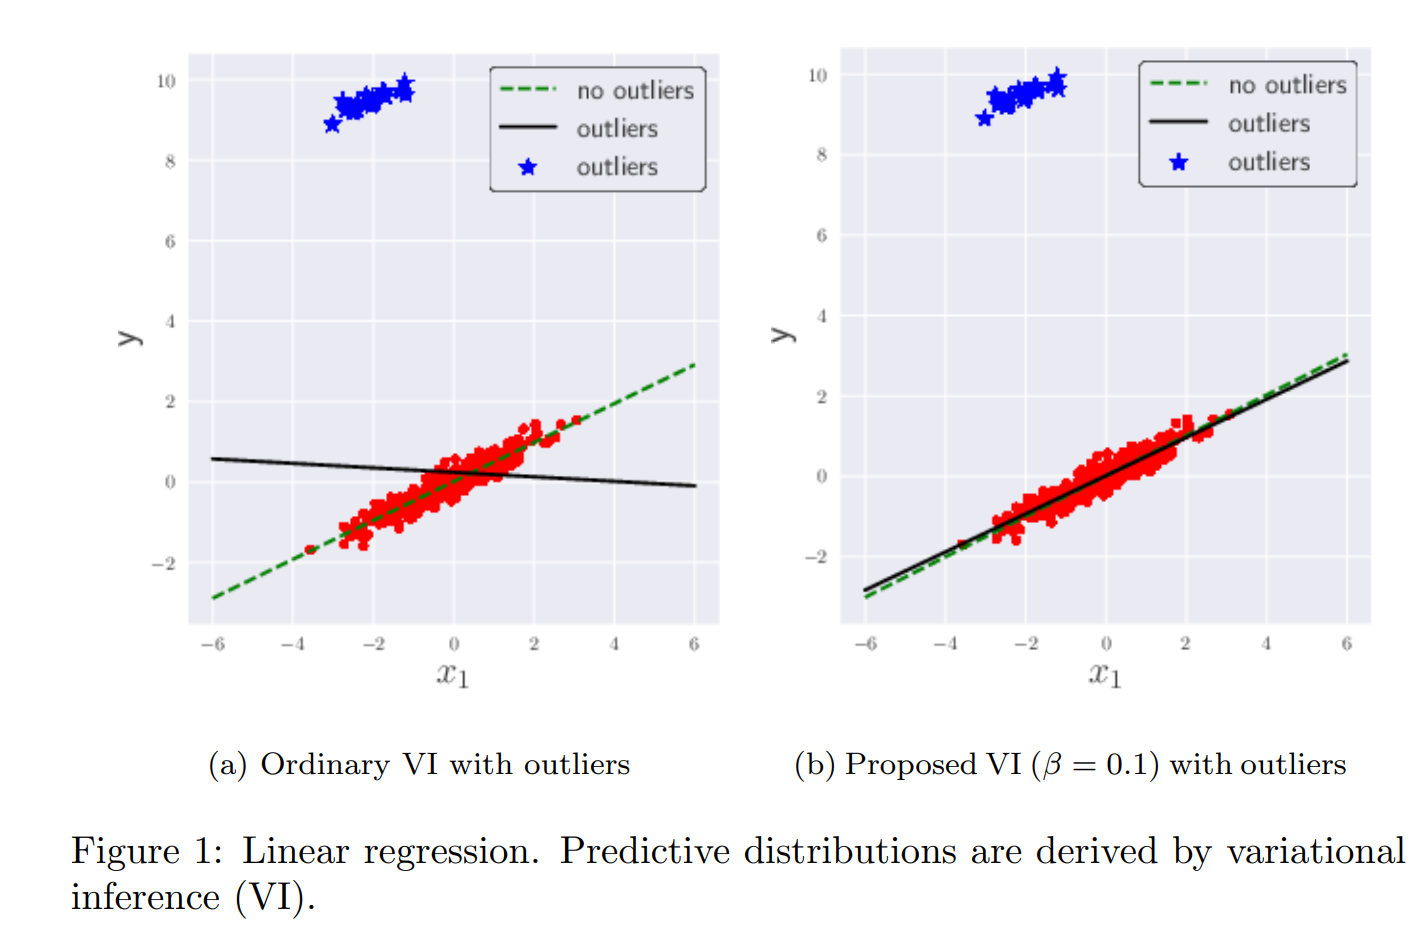
\includegraphics[width=\textwidth]{linreg.png}
\end{column}
\begin{column}{0.48\textwidth}
\textbf{Authors' Results:}
\begin{itemize}
    \item[\alert{$\times$}] \textbf{Ordinary VI:} predictive distribution \alert{heavily affected} by outliers
    \begin{itemize}
        \item Regression line pulled toward outliers
        \item Wide uncertainty bands
    \end{itemize}
    \item[\textcolor{green}{\checkmark}] \textbf{Proposed $\beta$-VI:} predictive distribution \alert{less affected} by outliers
    \begin{itemize}
        \item Regression line stable
        \item Confidence interval excludes outliers
    \end{itemize}
\end{itemize}
\end{column}
\end{columns}

\vspace{0.3cm}

\textbf{Key Mechanism:} $\beta$-divergence downweights outliers via $p(x_i|\theta)^\beta$
\[
\text{Outlier weight} = p(x_{\text{outlier}}|\theta)^\beta \ll p(x_{\text{inlier}}|\theta)^\beta \approx 1
\]

\textbf{Conclusion:} Even on simple linear model, robust divergence \alert{automatically suppresses} anomalous points while preserving inlier information

\end{frame}


\begin{frame}{Toy Experiment: Logistic Regression (Section 5.1)}

\begin{columns}
\begin{column}{0.52\textwidth}
\centering
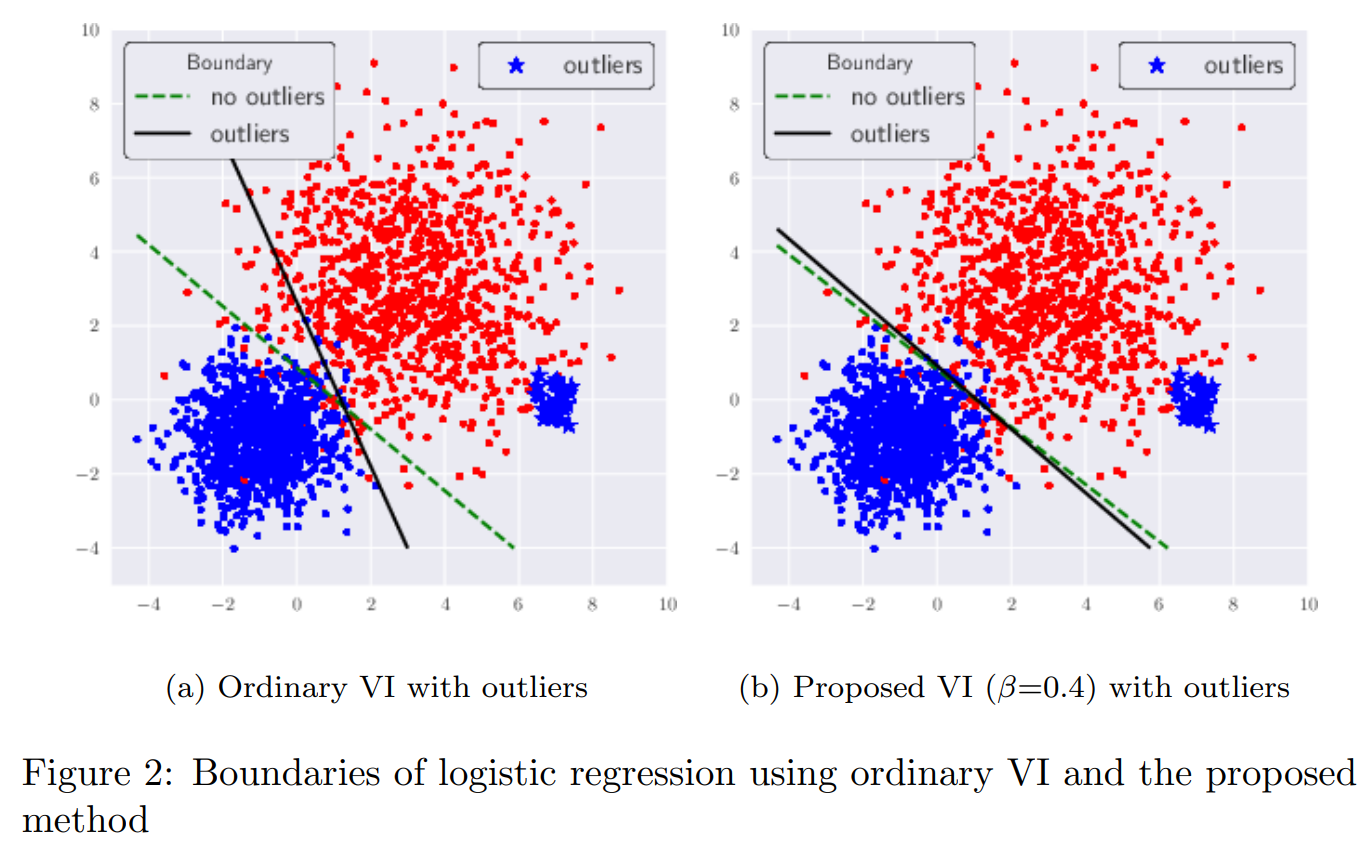
\includegraphics[width=\textwidth]{logreg.png}

\vspace{0.2cm}
\end{column}
\begin{column}{0.46\textwidth}
\textbf{Task:} Binary classification \\
\textbf{Outliers:} Wrongly labeled points

\vspace{0.0cm}

\textbf{Results:}
\begin{itemize}
    \item Ordinary VI: boundary \alert{heavily distorted}
    \item $\beta$-VI: boundary \textcolor{green}{stable}, clean separation
\end{itemize}

\vspace{+0.2cm}

\textbf{Mechanism:}
\[
p(y_{\text{wrong}}|x, \theta)^\beta \to 0
\]
Mislabeled points get near-zero weight
\end{column}
\end{columns}

\vspace{+0.1cm}

\textbf{Conclusion:} Visual confirmation of robustness to \alert{output-related outliers} (label noise) — critical for real-world classification tasks with annotation errors

\end{frame}


\end{document}
